



%%%%%%%%%%%%%%%%%%%%%%%%%%%%%%%%%%%%%%%%%
% Beamer Presentation
% LaTeX Template
% Version 1.0 (10/11/12)
%
% This template has been downloaded from:
% http://www.LaTeXTemplates.com
%
% License:
% CC BY-NC-SA 3.0 (http://creativecommons.org/licenses/by-nc-sa/3.0/)
%
%%%%%%%%%%%%%%%%%%%%%%%%%%%%%%%%%%%%%%%%%

%----------------------------------------------------------------------------------------
%	PACKAGES AND THEMES
%----------------------------------------------------------------------------------------

\documentclass[aspectratio=169]{beamer}

\mode<presentation> {


% The Beamer class comes with a number of default slide themes
% which change the colors and layouts of slides. Below this is a list
% of all the themes, uncomment each in turn to see what they look like.

%\usetheme{default}
%\usetheme{AnnArbor}
%\usetheme{Antibes}
%\usetheme{Bergen}
%\usetheme{Berkeley}
%\usetheme{Berlin}
%\usetheme{Boadilla}
%\usetheme{CambridgeUS}
%\usetheme{Copenhagen}
%\usetheme{Darmstadt}
%\usetheme{Dresden}
%\usetheme{Frankfurt}
%\usetheme{Goettingen}
%\usetheme{Hannover}
%\usetheme{Ilmenau}
%\usetheme{JuanLesPins}
%\usetheme{Luebeck}
\usetheme{Madrid}
%\usetheme{Malmoe}
%\usetheme{Marburg}
%\usetheme{Montpellier}
%\usetheme{PaloAlto}
%\usetheme{Pittsburgh}
%\usetheme{Rochester}
%\usetheme{Singapore}
%\usetheme{Szeged}
%\usetheme{Warsaw}

% As well as themes, the Beamer class has a number of color themes
% for any slide theme. Uncomment each of these in turn to see how it
% changes the colors of your current slide theme.

%\usecolortheme{albatross}
%\usecolortheme{beaver}
%\usecolortheme{beetle}
%\usecolortheme{crane}
%\usecolortheme{dolphin}
%\usecolortheme{dove}
%\usecolortheme{fly}
%\usecolortheme{lily}
%\usecolortheme{orchid}
%\usecolortheme{rose}
%\usecolortheme{seagull}
%\usecolortheme{seahorse}
%\usecolortheme{whale}
%\usecolortheme{wolverine}

%\setbeamertemplate{footline} % To remove the footer line in all slides uncomment this line
%\setbeamertemplate{footline}[page number] % To replace the footer line in all slides with a simple slide count uncomment this line

\definecolor{UOSred}{rgb}{0.6745098039215686, 0.02352941176470588, 0.2039215686274510} % UBC Blue (primary)
\definecolor{UOSgrey}{rgb}{0.8117647058823529, 0.8117647058823529, 0.8117647058823529} % UBC Grey (secondary)

\setbeamercolor{palette primary}{bg=UOSred,fg=white}
\setbeamercolor{palette secondary}{bg=UOSred,fg=white}
\setbeamercolor{palette tertiary}{bg=UOSred,fg=white}
\setbeamercolor{palette quaternary}{bg=UOSred,fg=white}
\setbeamercolor{structure}{fg=UOSred} % itemize, enumerate, etc
\setbeamercolor{section in toc}{fg=UOSred} % TOC sections

%gets rid of bottom navigation bars
\setbeamertemplate{footline}[frame number]{}

%gets rid of bottom navigation symbols
\setbeamertemplate{navigation symbols}{}


\usepackage{amsmath}
\usepackage{selinput}      % Halbautomatische Auswahl der Eingabecodierung
\SelectInputMappings{      % mit Hilfe ausgewählter Glyphen
  adieresis={ä},	   % siehe: http://partners.adobe.com/public/developer/en/opentype/glyphlist.txt
  germandbls={ß},
  Euro={€}
}

\addtobeamertemplate{footline}{%
  \leavevmode%
  \hbox{%
  \begin{beamercolorbox}[wd=\paperwidth,ht=2.25ex,dp=1ex,center]{author in head/foot}%
     \insertsectionnavigationhorizontal{\paperwidth}{}{}
  \end{beamercolorbox}}%

}

% Override palette coloring with secondary
\setbeamercolor{subsection in head/foot}{bg=UOSgrey,fg=white}

%\setbeamertemplate{navigation symbols}{} % To remove the navigation symbols from the bottom of all slides uncomment this line
}
\usepackage{hyperref}
\usepackage{graphicx} % Allows including images
\usepackage{grffile}
\usepackage{booktabs} % Allows the use of \toprule, \midrule and \bottomrule in tables
\graphicspath{{images/}}
%----------------------------------------------------------------------------------------
%	TITLE PAGE
%----------------------------------------------------------------------------------------

\title[Übungsprojekt Phase 3]{Übungsprojekt Phase 3} % The short title appears at the bottom of every slide, the full title is only on the title page

\author{T. Adam, M. ben Ahmed} % Your name
\institute[UOS] % Your institution as it will appear on the bottom of every slide, may be shorthand to save space
{

Universität Osnabrück \\ % Your institution for the title page

\medskip
\textit{Æ} % Your email address


}
\date{\today} % Date, can be changed to a custom date

\begin{document}

\begin{frame}
\titlepage % Print the title page as the first slide
\end{frame}


%----------------------------------------------------------------------------------------
%	PRESENTATION SLIDES
%----------------------------------------------------------------------------------------


%------------------------------------------------

\begin{frame}
	\frametitle{(a) - Basis-ILP}
	\textbf{Formulierung des Basis-ILP}\\
	\begin{itemize}
		\item $N$	= $ \{1,\dotsc,n\}$ := Punktmenge.
		\item $P$ = $ \{1,2,3,4\}$ := Labelpositionen.
		\item $o_{iajb} = 1$, wenn die Label von Punkt $i$ und $j$ in Positionen $a$ und $b$ überlappen, $0$ sonst.
		\item $l_{ia} = 1$, wenn Punkt $i$ in Position $a$ gelabelt ist, 0 sonst.
	\end{itemize}
	\end{frame}
%------------------------------------------------


\begin{frame}
	\frametitle{(a) - Basis-ILP}
	\textbf{Formulierung des Basis-ILP}

	\begin{align}
	\max     && \sum_{i = 1}^n \sum_{a = 1}^4 l_{ia} \\
	\text{s.t.}
					&& \sum_{a = 1}^4 l_{ia} \leq 1                    && \forall i \in N\\
					&&   o_{iajb} + l_{ia} + l_{jb} \leq  2        && \forall a,b \in P,\thinspace \thinspace \forall i,j\in N : i \neq j \\
					&&   l_{ia} \in \{0,1\}                            && \forall a \in P,\thinspace \thinspace \forall i\in N                                      
	\end{align}
	\\
	(1) Maximiere die Anzahl der gelabelten Punkte.\\
	(2) Pro Punkt darf maximal eine Labelposition gewählt werden.\\
	(3) Wenn sich Label von zwei Punkten überlappen, darf maximal ein Punkt gelabelt werden.\\
	(4) Variable $l_{ia}$ ist binär.
	\end{frame}
%------------------------------------------------
\begin{frame}
	\frametitle{(d) Ergebnisse - Testmaschinen}
	\begin{columns}[c] % The "c" option specifies centered vertical alignment while the "t" option is used for top vertical alignment
		
		\column{.30\textwidth} % Left column and width
		\textbf{Intel Core i5-3570K}
		\begin{itemize}
			\item 4c/4t
			\item 3,4 - 3,8 GHz
			\item 6 MB L3
			\item 16 GB (1600 MHz)
			\item Linux (Kubuntu 18.04)
			
		\end{itemize}
		
		\column{.30\textwidth} % Right column and width
		\textbf{Intel Core i7-3770K}
		\begin{itemize}
			\item 4c/8t
			\item 3,5 - 3,9 GHz
			\item 8 MB L3
			\item 16 GB (1600 MHz)
			\item Linux (Kubuntu 18.04)
			
		\end{itemize}
	
	\end{columns}
	\end{frame}
	
	%------------------------------------------------


\begin{frame}
	\frametitle{(d) Ergebnisse - Heuristiken vs. ILP}
	\textbf{Vergleich der gelabelten Punkte}
	\begin{columns}[c] % The "c" option specifies centered vertical alignment while the "t" option is used for top vertical alignment
	
	\column{.45\textwidth} % Right column and width
	
	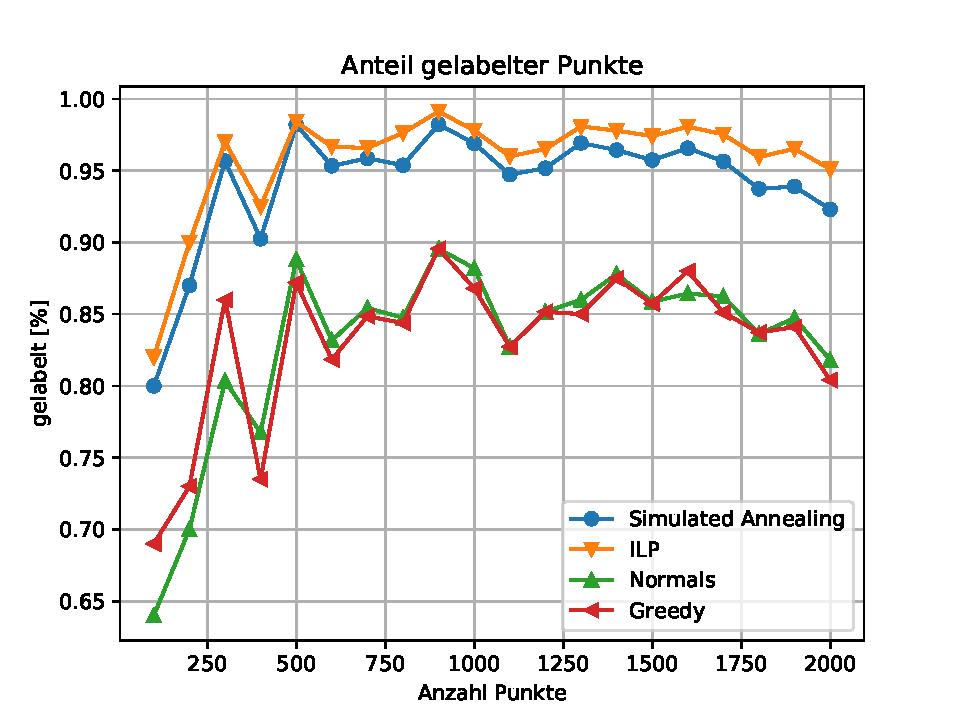
\includegraphics[scale=.45]{gelabelt_all.pdf}
	\column{.45\textwidth} % Left column and width
	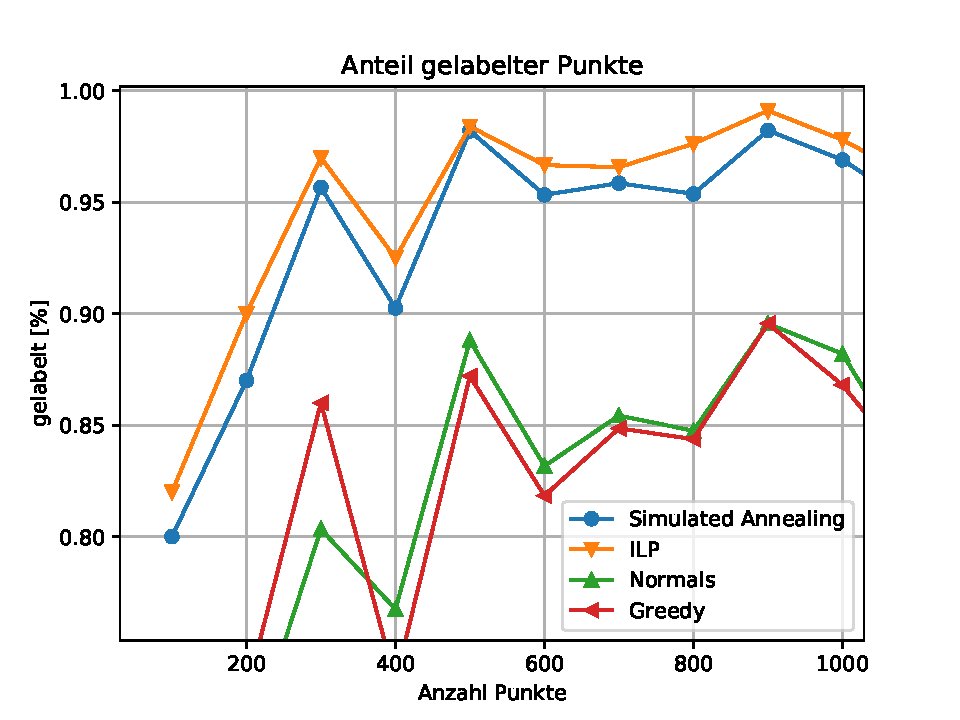
\includegraphics[scale=.45]{gelabelt_detail.pdf}
	

	\end{columns}

	\end{frame}

%------------------------------------------------


\begin{frame}
	\frametitle{(d) Ergebnisse - Heuristiken vs. ILP}
	\textbf{Vergleich der Laufzeiten}
	\begin{columns}[c] % The "c" option specifies centered vertical alignment while the "t" option is used for top vertical alignment
	
	\column{.45\textwidth} % Right column and width
	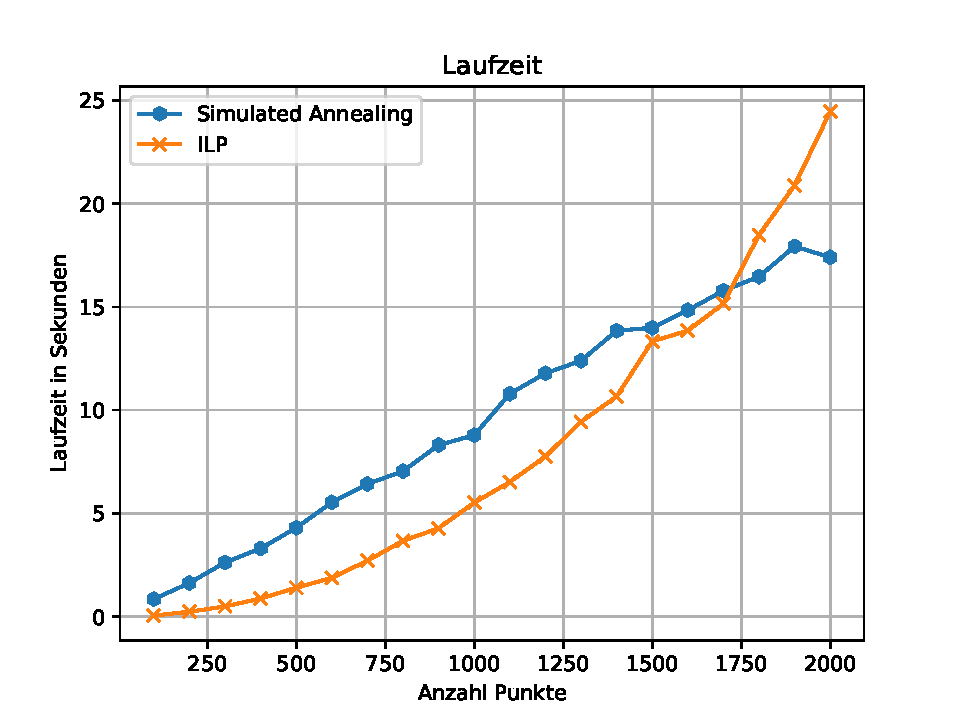
\includegraphics[scale=.45]{laufzeit_sa_ilp.pdf}
	
	\column{.45\textwidth} % Left column and width
	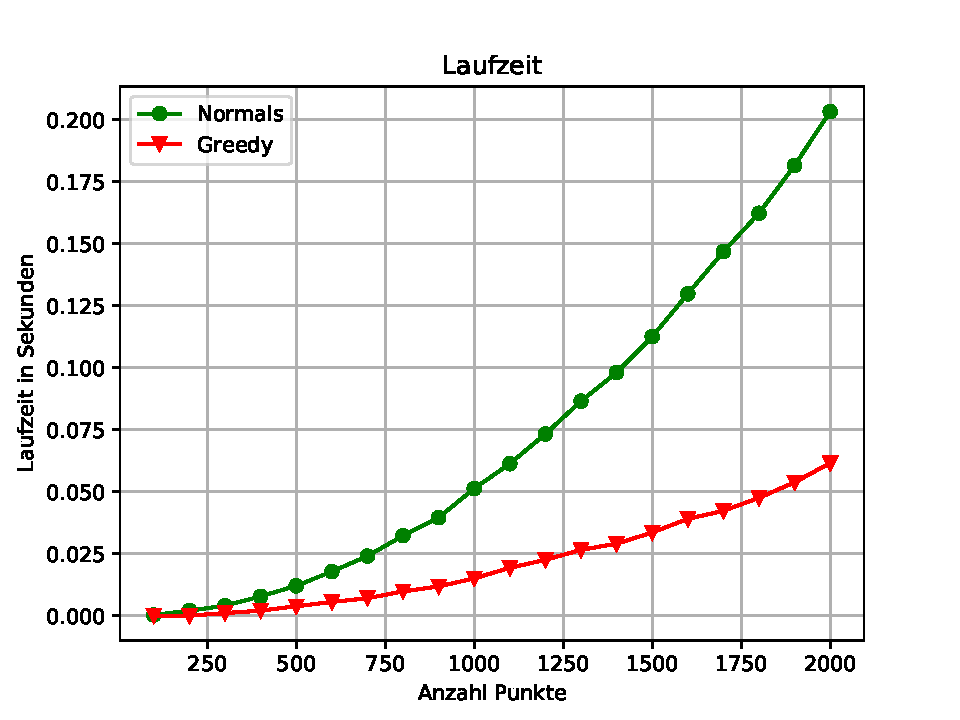
\includegraphics[scale=.45]{laufzeit_normals_greedy.pdf}
	
	

	\end{columns}

	\end{frame}

%------------------------------------------------

\begin{frame}
	\frametitle{(d) Ergebnisse - Heuristiken vs. ILP}
	\textbf{Vergleich des Speicherverbrauchs}
	\begin{columns}[c] % The "c" option specifies centered vertical alignment while the "t" option is used for top vertical alignment
	
	\column{.45\textwidth} % Right column and width
	
	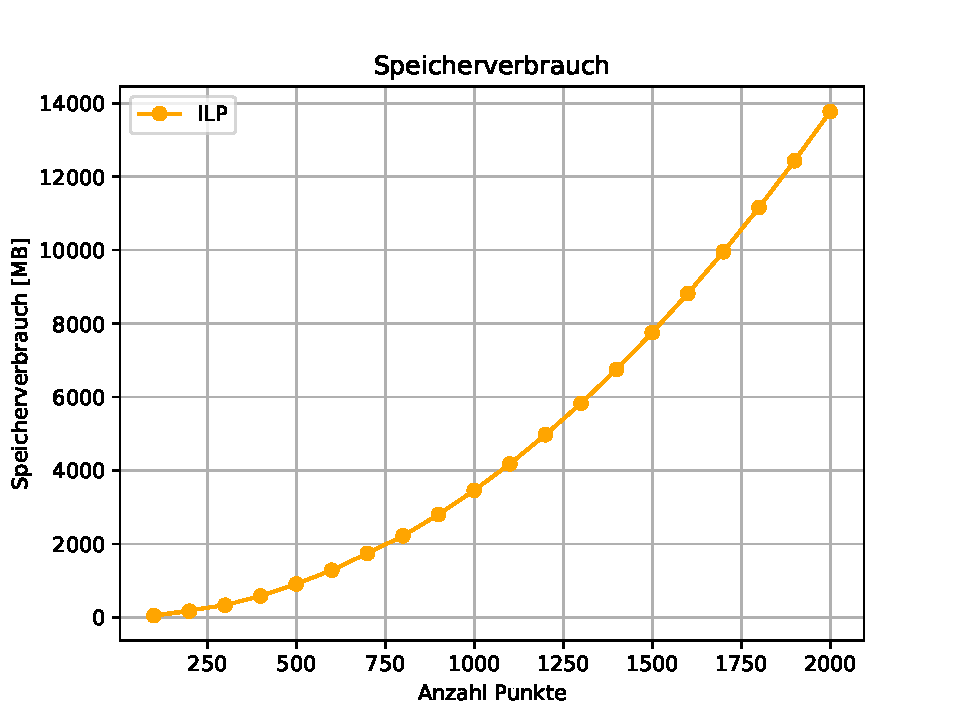
\includegraphics[scale=.45]{speicher_ilp.pdf}
	\column{.45\textwidth} % Left column and width
	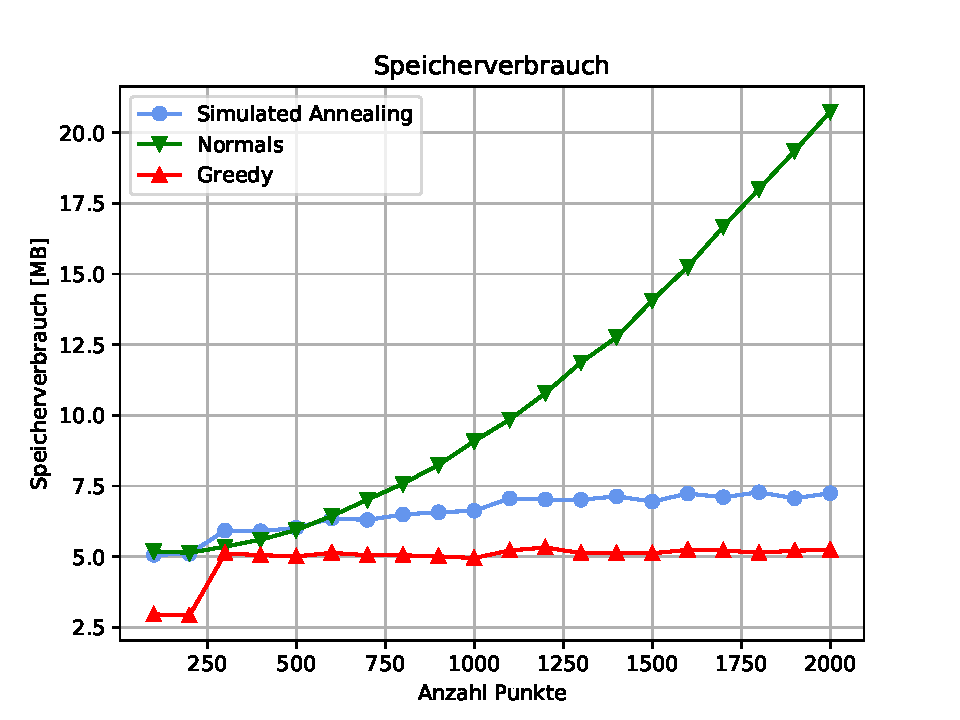
\includegraphics[scale=.45]{speicher_heuristiken.pdf}
	
	

	\end{columns}

	\end{frame}

%------------------------------------------------

\begin{frame}
	\frametitle{(d) Ergebnisse - ILP Verbesserungen}
	\begin{columns}[c] % The "c" option specifies centered vertical alignment while the "t" option is used for top vertical alignment
	
	\column{.5\textwidth} % Right column and width
	\textbf{}\\
	Einfluss der Verbesserungen auf die Laufzeit des ILP-Solvers
	
	
	\column{.45\textwidth} % Left column and width
	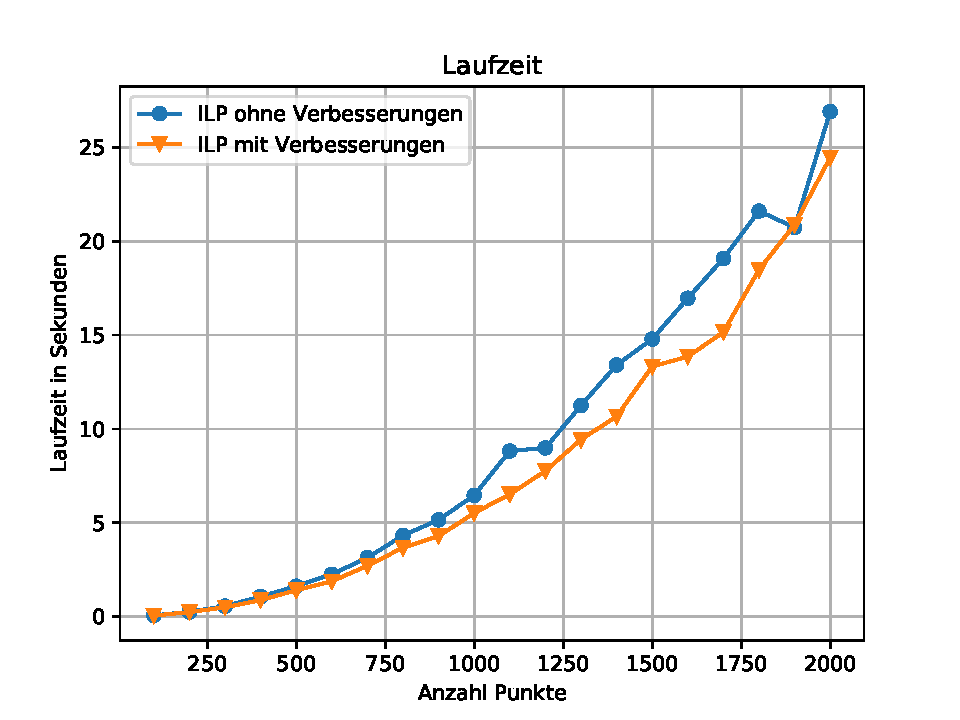
\includegraphics[scale=.45]{laufzeit_ilp_verbesserung.pdf}
	

	\end{columns}
	\end{frame}

%------------------------------------------------



\end{document} 